\documentclass[PredictiveAnalytics101.tex]{subfiles} 
\begin{document} 
%==============================================%


% Graphical Methods
% ROC Curves
% Lift
%==============================================%
\begin{frame}
\frametitle{ROC curves}

\begin{itemize}
\item
\item
\end{itemize}
\end{frame}
%==============================================%
\begin{frame}
\begin{figure}
\centering
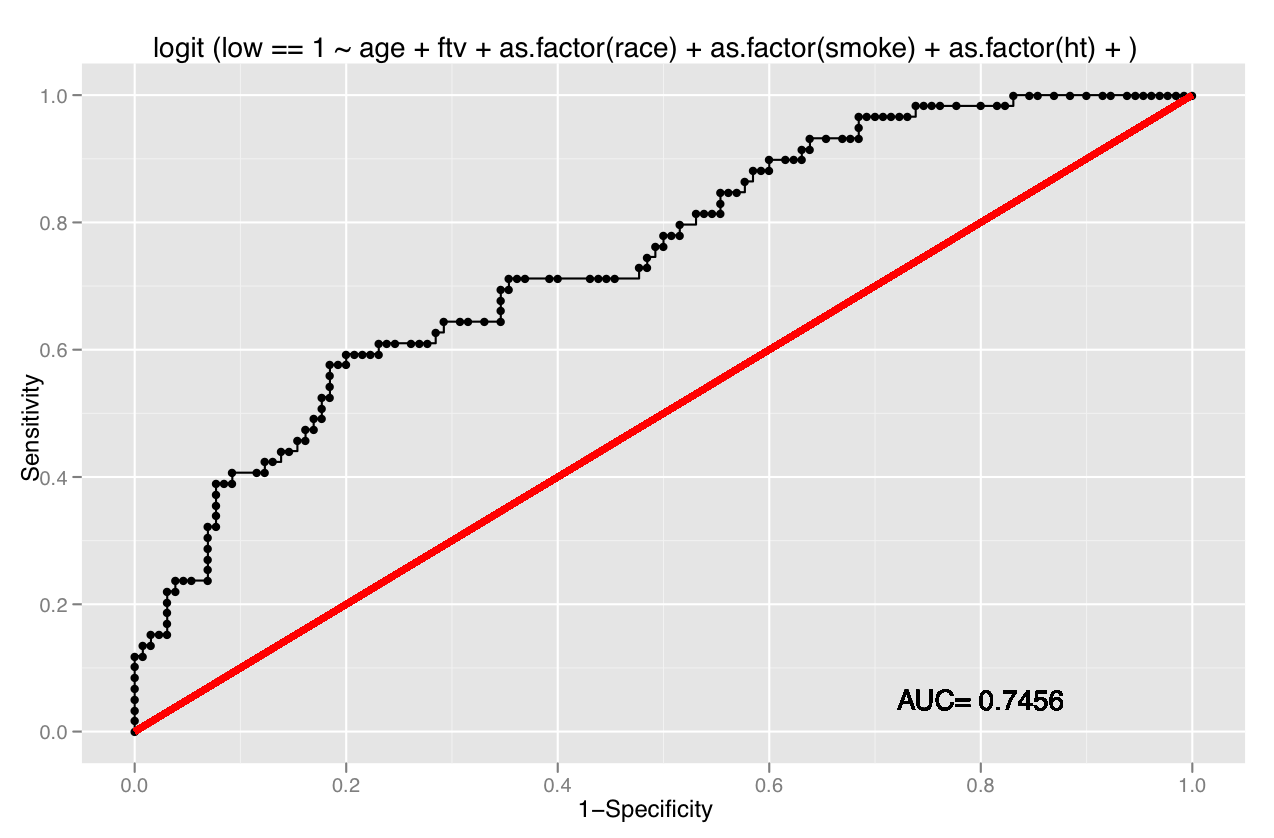
\includegraphics[width=0.7\linewidth]{LROCPlot}

\end{figure}
\end{frame}
%==============================================%
\begin{frame}
	AUC or Area Under the Curve is a single numerical measure of predictive power.
\begin{figure}
\centering
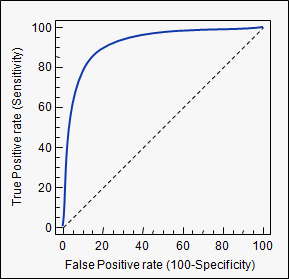
\includegraphics[width=0.7\linewidth]{ROC1}
\end{figure}
	
	
\end{frame}
\end{document}